\begin{document}

\chapter[Testbed]{Testbed}
\chaptermark{Testbed}
\label{chap:Testbed}
This is a section, where LaTeX functionality can be tested!
\section{Graphics}
\subsection{Including .eps-files}

\begin{figure}[H]
\centering
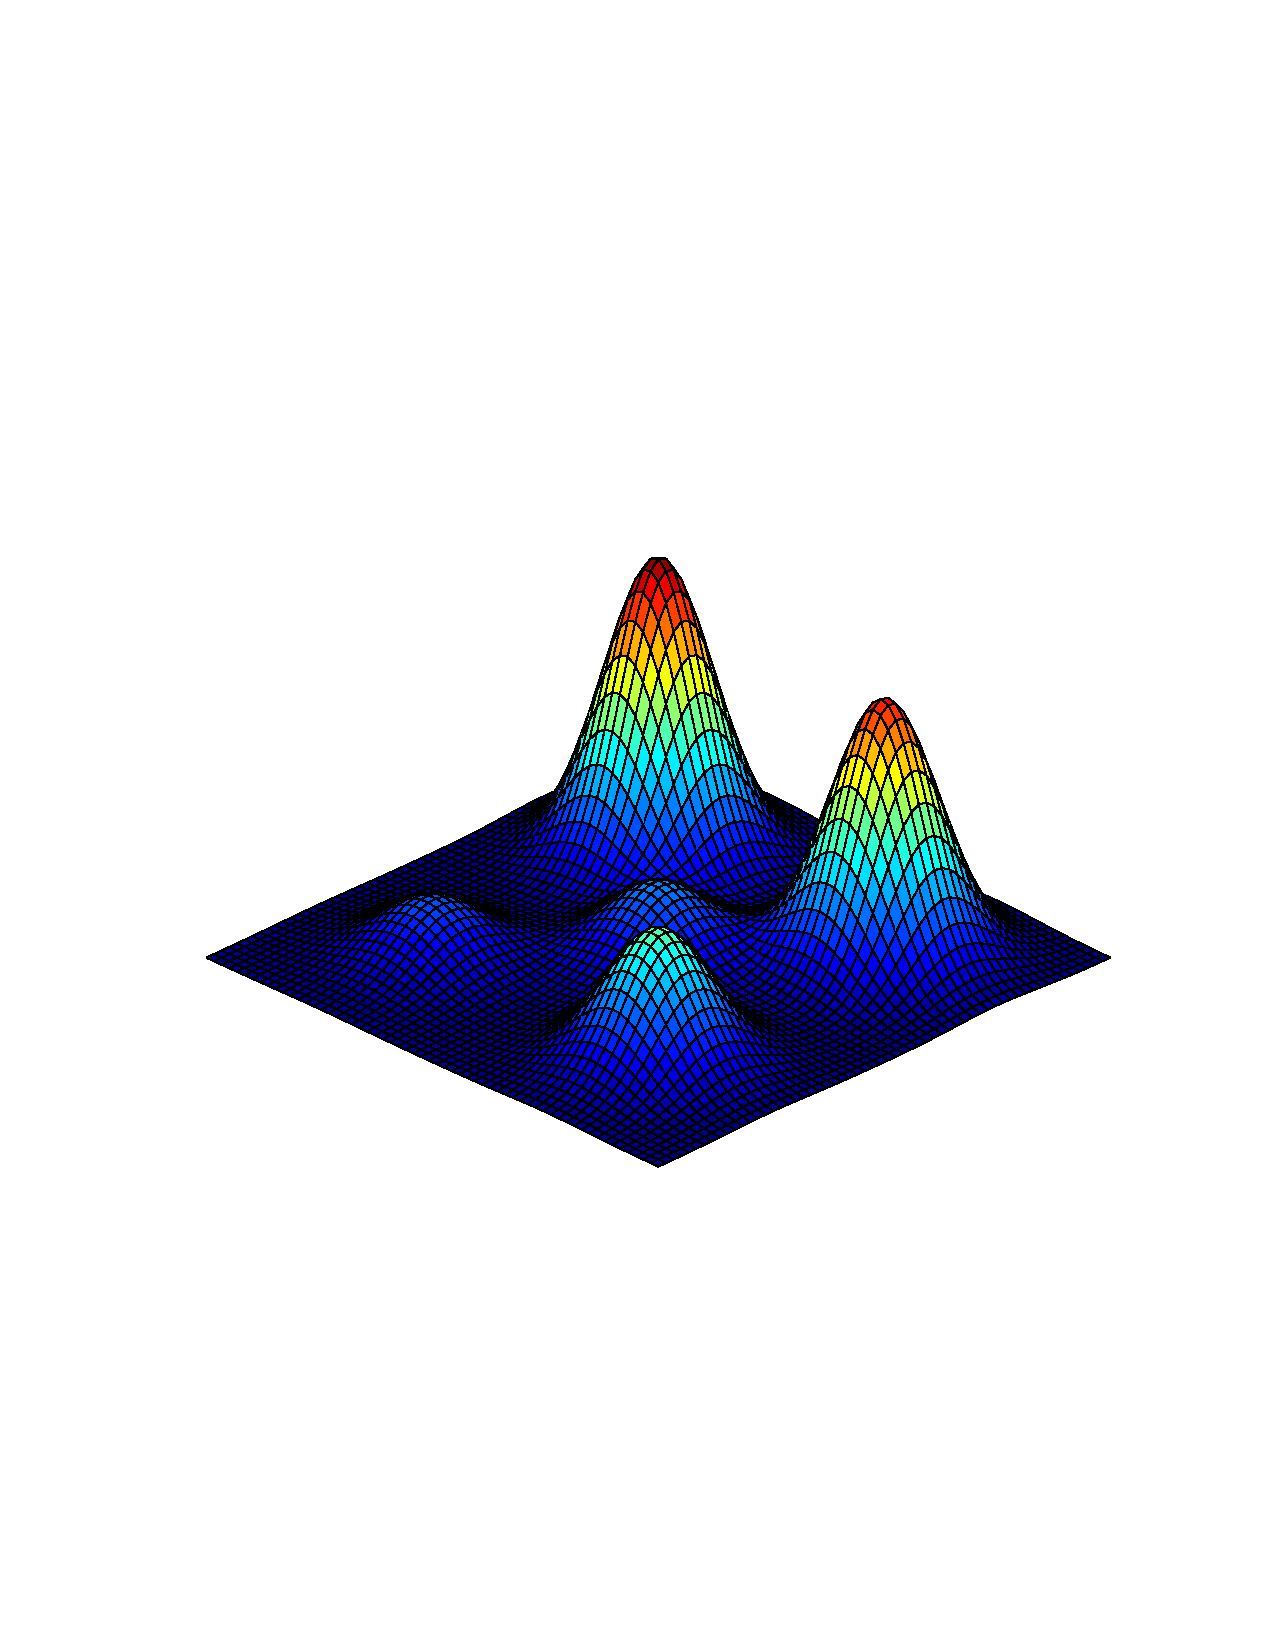
\includegraphics[width=0.5\textwidth]{gaussian}
\caption{Multiple three-dimensional gaussian distributions...}
\label{fig:mog}
\end{figure}


This is the text beneath an included picture. Figure \ref{fig:mog} shows an example of how to include eps-figures in this document.

\subsubsection{Displaying two eps-figures side-by-side}
\begin{figure}[H]
 \centering
 \begin{subfigure}{0.49\textwidth}
    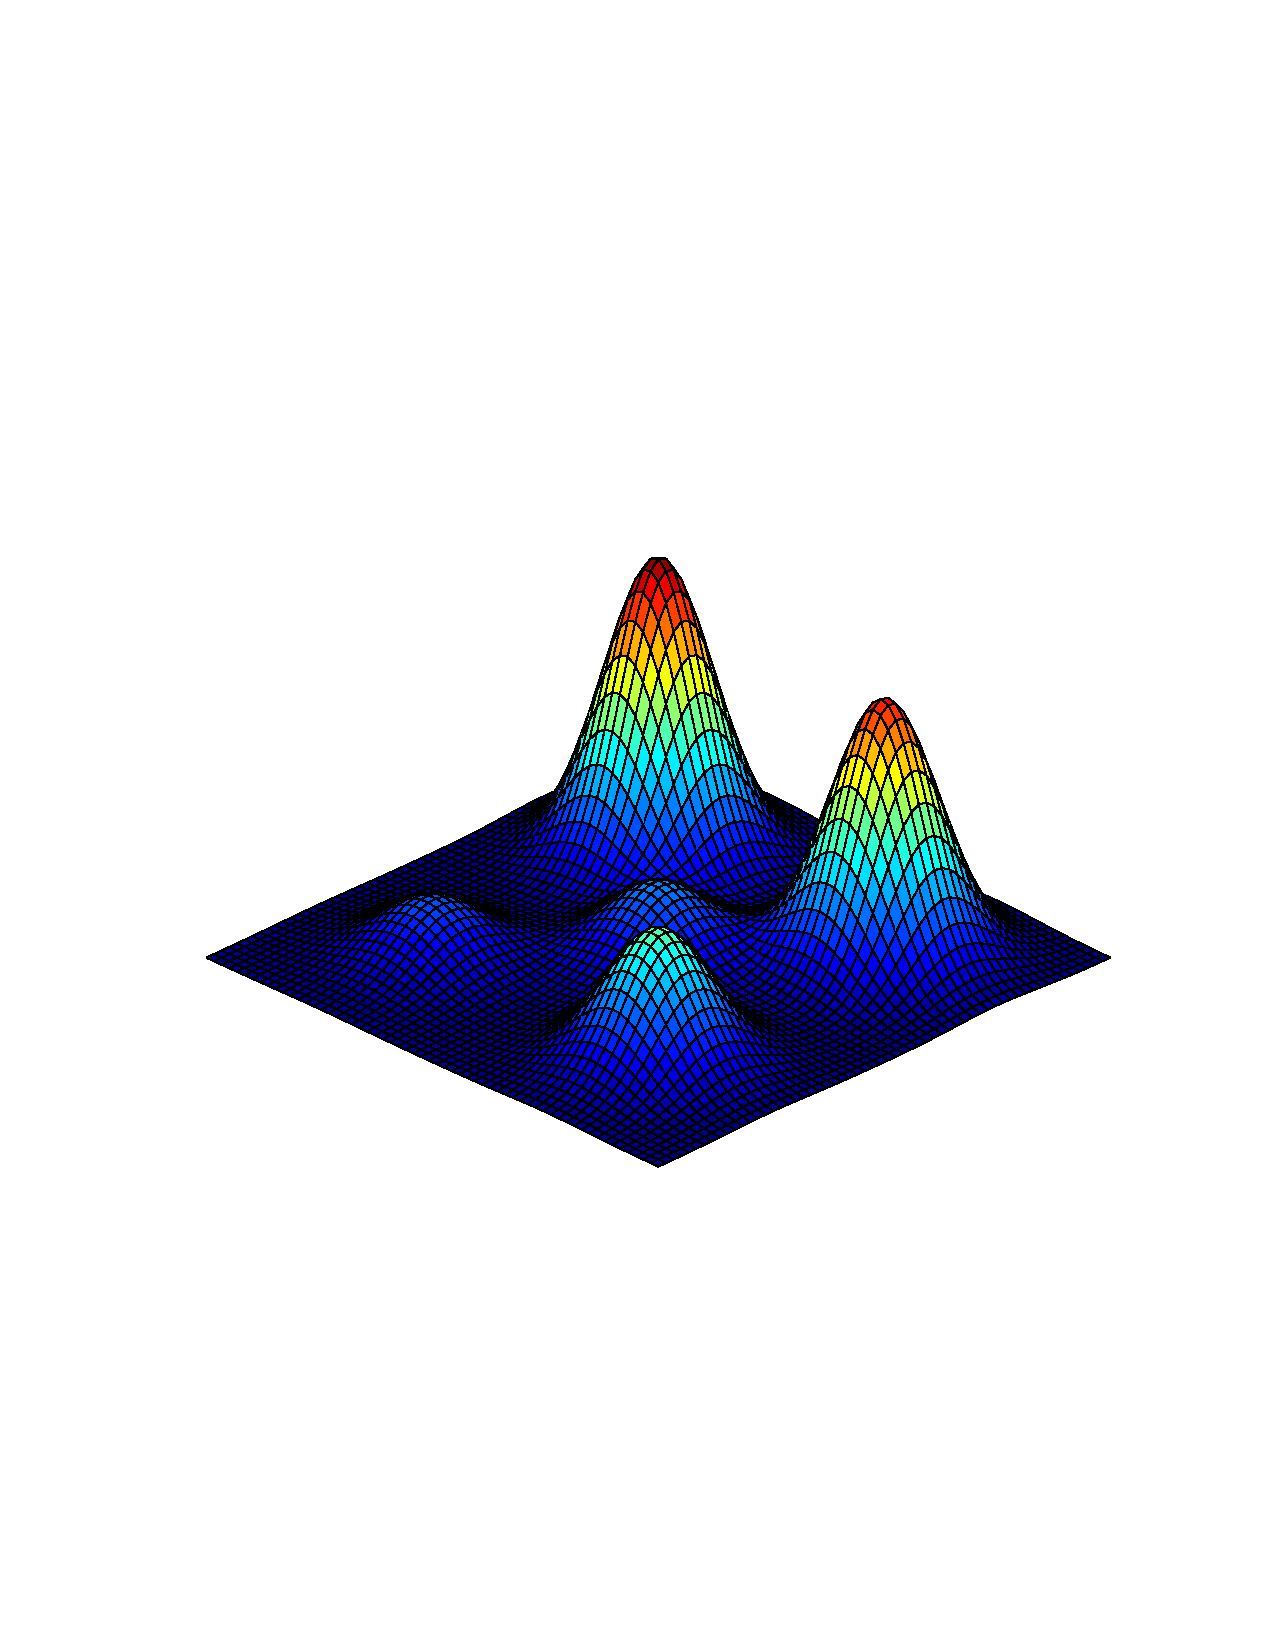
\includegraphics[width=\textwidth]{gaussian}
    \caption{Sub caption}
 \end{subfigure}
 \begin{subfigure}{0.49\textwidth}
    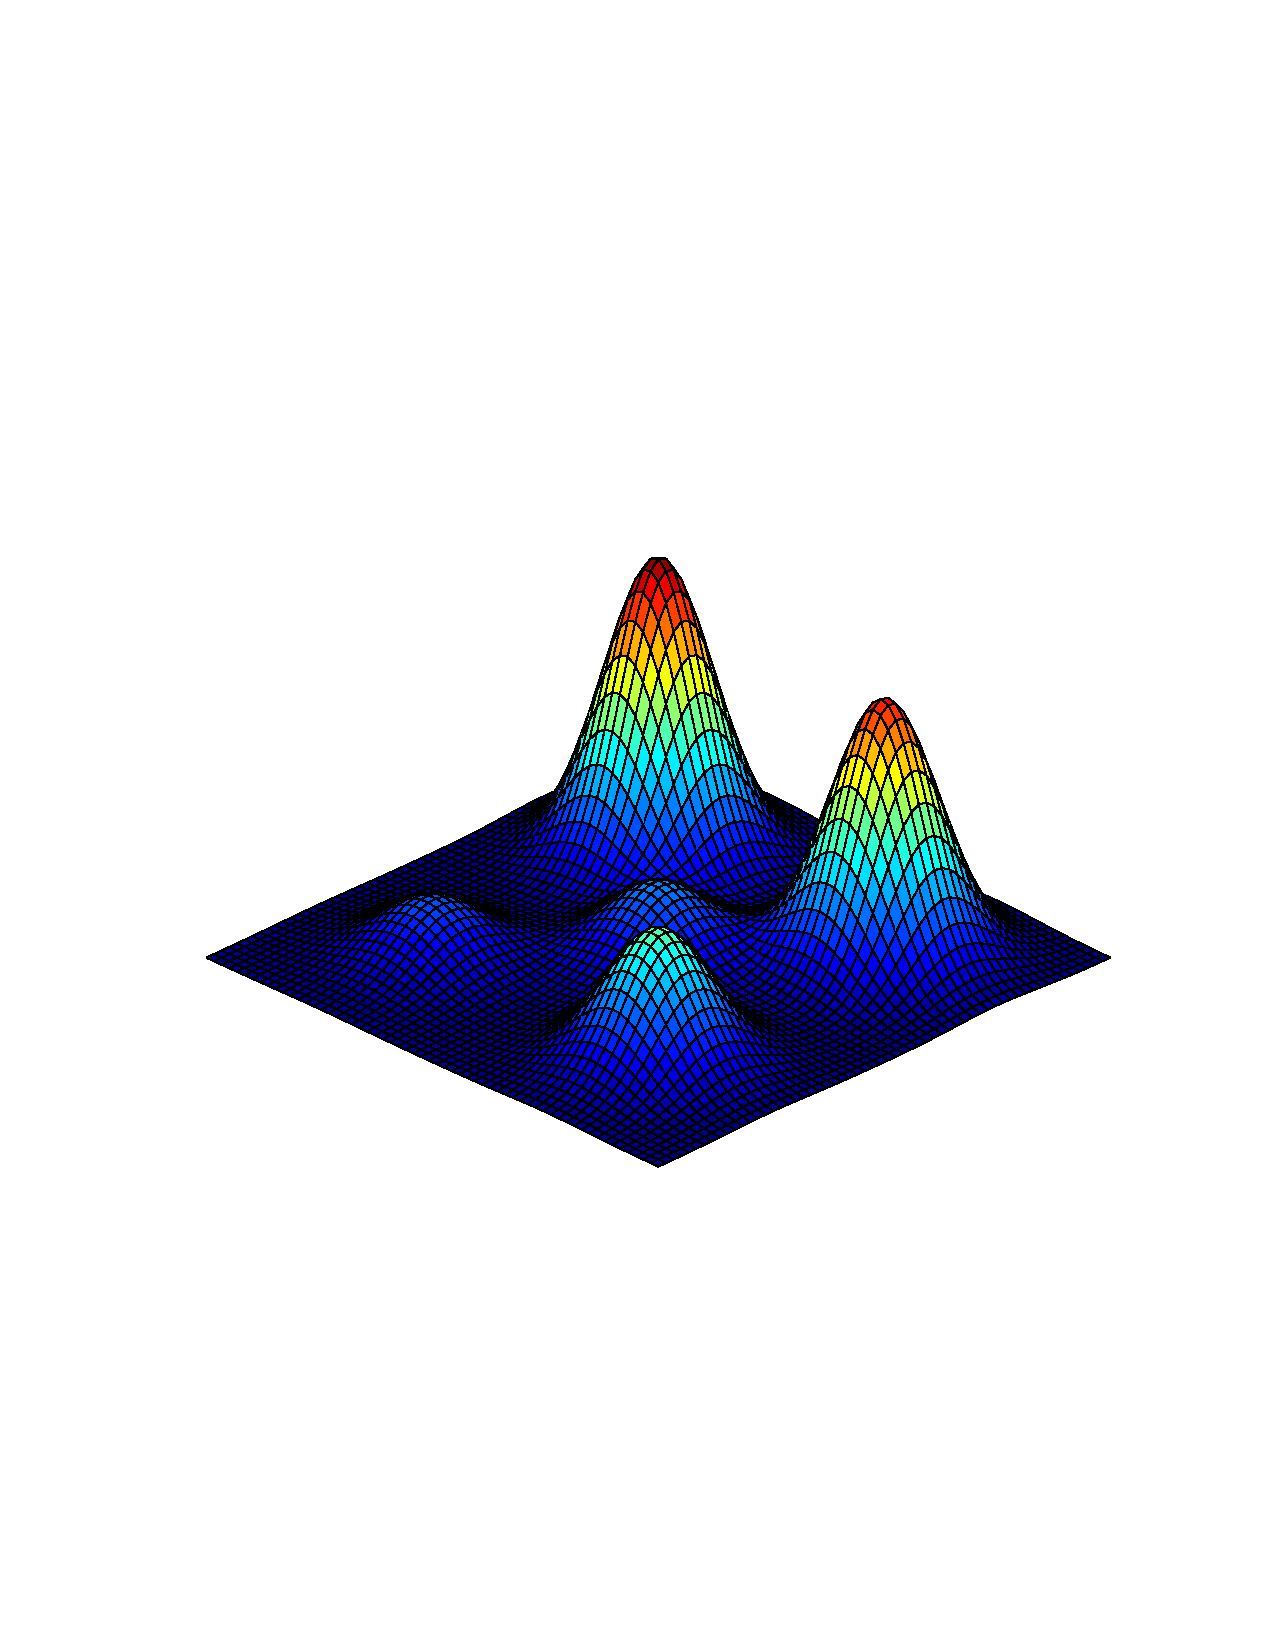
\includegraphics[width=\textwidth]{gaussian}
    \caption{Sub caption}
 \end{subfigure}
 \caption{Main caption}
\end{figure}

\subsection{Including tikz-figures}
\subsubsection{Two-dimensional figures}
Graphs can be included, like is shown in figure \ref{fig:sin}, using the input-method.
\tikzset{every picture/.style={scale=0.9}}
\begin{figure}[H]
	\centering
	% This file was created by matlab2tikz.
%
%The latest updates can be retrieved from
%  http://www.mathworks.com/matlabcentral/fileexchange/22022-matlab2tikz-matlab2tikz
%where you can also make suggestions and rate matlab2tikz.
%
\definecolor{mycolor1}{rgb}{0.00000,0.44700,0.74100}%
%
\begin{tikzpicture}

\begin{axis}[%
width=6.028in,
height=4.754in,
at={(1.011in,0.642in)},
scale only axis,
xmin=0,
xmax=6.28318530717959,
xtick={0,1.5707963267949,3.14159265358979,4.71238898038469,6.28318530717959},
xticklabels={{0},{$\text{1/2 }\pi$},{$\pi$},{$\text{3/2 }\pi$},{$\text{2}\pi$}},
ymin=-1.5,
ymax=1.5,
ytick={-1,  0,  1},
axis background/.style={fill=white}
]
\addplot [color=mycolor1, forget plot]
  table[row sep=crcr]{%
0	0\\
0.126933036508679	0.126592453573749\\
0.253866073017357	0.251147987181079\\
0.380799109526036	0.371662455660328\\
0.507732146034714	0.486196736100469\\
0.634665182543393	0.59290792905464\\
0.761598219052071	0.690079011482112\\
0.88853125556075	0.776146464291757\\
1.01546429206943	0.849725429949514\\
1.14239732857811	0.909631995354518\\
1.26933036508679	0.954902241444074\\
1.39626340159546	0.984807753012208\\
1.52319643810414	0.998867339183008\\
1.65012947461282	0.996854775951942\\
1.7770625111215	0.978802446214779\\
1.90399554763018	0.945000818714669\\
2.03092858413886	0.895993774291336\\
2.15786162064753	0.832569854634771\\
2.28479465715621	0.755749574354258\\
2.41172769366489	0.666769000516292\\
2.53866073017357	0.567059863862771\\
2.66559376668225	0.458226521727411\\
2.79252680319093	0.342020143325669\\
2.91945983969961	0.220310532786541\\
3.04639287620828	0.0950560433041829\\
3.17332591271696	-0.0317279334980679\\
3.30025894922564	-0.15800139597335\\
3.42719198573432	-0.281732556841429\\
3.554125022243	-0.400930535406613\\
3.68105805875168	-0.513677391573406\\
3.80799109526036	-0.618158986220605\\
3.93492413176903	-0.712694171378863\\
4.06185716827771	-0.795761840530832\\
4.18879020478639	-0.866025403784438\\
4.31572324129507	-0.922354294104581\\
4.44265627780375	-0.963842158559942\\
4.56958931431243	-0.989821441880933\\
4.69652235082111	-0.999874127673875\\
4.82345538732978	-0.993838464461254\\
4.95038842383846	-0.971811568323542\\
5.07732146034714	-0.934147860265107\\
5.20425449685582	-0.881453363447582\\
5.3311875333645	-0.814575952050336\\
5.45812056987318	-0.734591708657534\\
5.58505360638185	-0.64278760968654\\
5.71198664289053	-0.540640817455597\\
5.83891967939921	-0.429794912089172\\
5.96585271590789	-0.312033445698487\\
6.09278575241657	-0.189251244360411\\
6.21971878892525	-0.0634239196565654\\
6.34665182543393	0.0634239196565649\\
6.4735848619426	0.18925124436041\\
6.60051789845128	0.312033445698487\\
6.72745093495996	0.429794912089172\\
6.85438397146864	0.540640817455597\\
6.98131700797732	0.642787609686539\\
7.108250044486	0.734591708657533\\
7.23518308099467	0.814575952050335\\
7.36211611750335	0.881453363447582\\
7.48904915401203	0.934147860265107\\
7.61598219052071	0.971811568323542\\
7.74291522702939	0.993838464461254\\
7.86984826353807	0.999874127673875\\
7.99678130004675	0.989821441880933\\
8.12371433655542	0.963842158559942\\
8.2506473730641	0.922354294104582\\
8.37758040957278	0.866025403784439\\
8.50451344608146	0.795761840530832\\
8.63144648259014	0.712694171378863\\
8.75837951909882	0.618158986220606\\
8.88531255560749	0.513677391573407\\
9.01224559211617	0.400930535406613\\
9.13917862862485	0.28173255684143\\
9.26611166513353	0.158001395973351\\
9.39304470164221	0.031727933498067\\
9.51997773815089	-0.0950560433041828\\
9.64691077465957	-0.22031053278654\\
9.77384381116824	-0.342020143325668\\
9.90077684767692	-0.458226521727409\\
10.0277098841856	-0.567059863862771\\
10.1546429206943	-0.666769000516291\\
10.281575957203	-0.755749574354258\\
10.4085089937116	-0.832569854634771\\
10.5354420302203	-0.895993774291336\\
10.662375066729	-0.945000818714668\\
10.7893081032377	-0.978802446214779\\
10.9162411397464	-0.996854775951942\\
11.043174176255	-0.998867339183008\\
11.1701072127637	-0.984807753012208\\
11.2970402492724	-0.954902241444074\\
11.4239732857811	-0.909631995354518\\
11.5509063222897	-0.849725429949514\\
11.6778393587984	-0.776146464291757\\
11.8047723953071	-0.690079011482113\\
11.9317054318158	-0.59290792905464\\
12.0586384683245	-0.486196736100469\\
12.1855715048331	-0.371662455660328\\
12.3125045413418	-0.251147987181081\\
12.4394375778505	-0.126592453573751\\
12.5663706143592	-4.89858719658941e-16\\
};
\end{axis}
\end{tikzpicture}%
	\caption{A sine wave}
	\label{fig:sin}
\end{figure}

As figure \ref{fig:sin} was a little big, we now try to scale this output somehow:

\tikzset{every picture/.style={scale=0.6}}
\begin{figure}[H]
	\centering
	% This file was created by matlab2tikz.
%
%The latest updates can be retrieved from
%  http://www.mathworks.com/matlabcentral/fileexchange/22022-matlab2tikz-matlab2tikz
%where you can also make suggestions and rate matlab2tikz.
%
\definecolor{mycolor1}{rgb}{0.00000,0.44700,0.74100}%
%
\begin{tikzpicture}

\begin{axis}[%
width=6.028in,
height=4.754in,
at={(1.011in,0.642in)},
scale only axis,
xmin=0,
xmax=6.28318530717959,
xtick={0,1.5707963267949,3.14159265358979,4.71238898038469,6.28318530717959},
xticklabels={{0},{$\text{1/2 }\pi$},{$\pi$},{$\text{3/2 }\pi$},{$\text{2}\pi$}},
ymin=-1.5,
ymax=1.5,
ytick={-1,  0,  1},
axis background/.style={fill=white}
]
\addplot [color=mycolor1, forget plot]
  table[row sep=crcr]{%
0	0\\
0.126933036508679	0.126592453573749\\
0.253866073017357	0.251147987181079\\
0.380799109526036	0.371662455660328\\
0.507732146034714	0.486196736100469\\
0.634665182543393	0.59290792905464\\
0.761598219052071	0.690079011482112\\
0.88853125556075	0.776146464291757\\
1.01546429206943	0.849725429949514\\
1.14239732857811	0.909631995354518\\
1.26933036508679	0.954902241444074\\
1.39626340159546	0.984807753012208\\
1.52319643810414	0.998867339183008\\
1.65012947461282	0.996854775951942\\
1.7770625111215	0.978802446214779\\
1.90399554763018	0.945000818714669\\
2.03092858413886	0.895993774291336\\
2.15786162064753	0.832569854634771\\
2.28479465715621	0.755749574354258\\
2.41172769366489	0.666769000516292\\
2.53866073017357	0.567059863862771\\
2.66559376668225	0.458226521727411\\
2.79252680319093	0.342020143325669\\
2.91945983969961	0.220310532786541\\
3.04639287620828	0.0950560433041829\\
3.17332591271696	-0.0317279334980679\\
3.30025894922564	-0.15800139597335\\
3.42719198573432	-0.281732556841429\\
3.554125022243	-0.400930535406613\\
3.68105805875168	-0.513677391573406\\
3.80799109526036	-0.618158986220605\\
3.93492413176903	-0.712694171378863\\
4.06185716827771	-0.795761840530832\\
4.18879020478639	-0.866025403784438\\
4.31572324129507	-0.922354294104581\\
4.44265627780375	-0.963842158559942\\
4.56958931431243	-0.989821441880933\\
4.69652235082111	-0.999874127673875\\
4.82345538732978	-0.993838464461254\\
4.95038842383846	-0.971811568323542\\
5.07732146034714	-0.934147860265107\\
5.20425449685582	-0.881453363447582\\
5.3311875333645	-0.814575952050336\\
5.45812056987318	-0.734591708657534\\
5.58505360638185	-0.64278760968654\\
5.71198664289053	-0.540640817455597\\
5.83891967939921	-0.429794912089172\\
5.96585271590789	-0.312033445698487\\
6.09278575241657	-0.189251244360411\\
6.21971878892525	-0.0634239196565654\\
6.34665182543393	0.0634239196565649\\
6.4735848619426	0.18925124436041\\
6.60051789845128	0.312033445698487\\
6.72745093495996	0.429794912089172\\
6.85438397146864	0.540640817455597\\
6.98131700797732	0.642787609686539\\
7.108250044486	0.734591708657533\\
7.23518308099467	0.814575952050335\\
7.36211611750335	0.881453363447582\\
7.48904915401203	0.934147860265107\\
7.61598219052071	0.971811568323542\\
7.74291522702939	0.993838464461254\\
7.86984826353807	0.999874127673875\\
7.99678130004675	0.989821441880933\\
8.12371433655542	0.963842158559942\\
8.2506473730641	0.922354294104582\\
8.37758040957278	0.866025403784439\\
8.50451344608146	0.795761840530832\\
8.63144648259014	0.712694171378863\\
8.75837951909882	0.618158986220606\\
8.88531255560749	0.513677391573407\\
9.01224559211617	0.400930535406613\\
9.13917862862485	0.28173255684143\\
9.26611166513353	0.158001395973351\\
9.39304470164221	0.031727933498067\\
9.51997773815089	-0.0950560433041828\\
9.64691077465957	-0.22031053278654\\
9.77384381116824	-0.342020143325668\\
9.90077684767692	-0.458226521727409\\
10.0277098841856	-0.567059863862771\\
10.1546429206943	-0.666769000516291\\
10.281575957203	-0.755749574354258\\
10.4085089937116	-0.832569854634771\\
10.5354420302203	-0.895993774291336\\
10.662375066729	-0.945000818714668\\
10.7893081032377	-0.978802446214779\\
10.9162411397464	-0.996854775951942\\
11.043174176255	-0.998867339183008\\
11.1701072127637	-0.984807753012208\\
11.2970402492724	-0.954902241444074\\
11.4239732857811	-0.909631995354518\\
11.5509063222897	-0.849725429949514\\
11.6778393587984	-0.776146464291757\\
11.8047723953071	-0.690079011482113\\
11.9317054318158	-0.59290792905464\\
12.0586384683245	-0.486196736100469\\
12.1855715048331	-0.371662455660328\\
12.3125045413418	-0.251147987181081\\
12.4394375778505	-0.126592453573751\\
12.5663706143592	-4.89858719658941e-16\\
};
\end{axis}
\end{tikzpicture}%
	\caption{A second sine wave}
	\label{fig:sin2}
\end{figure}

We can also display more than one lineplot in one row:

\tikzset{every picture/.style={scale=0.5}}
\begin{figure}[H]
	\centering
	\begin{subfigure}{0.49\textwidth}
		\includestandalone[width=\textwidth]{plots/sin-tikz}
		\caption{A sine wave}
	\end{subfigure}
	\begin{subfigure}{0.49\textwidth}
		\includestandalone[width=\textwidth]{plots/cos-tikz}
		\caption{A cosine wave}
	\end{subfigure}
	\caption{Sine and cosine waves}
	\label{fig:sin}
\end{figure}

\subsubsection{Three-dimensional figures}
\tikzset{every picture/.style={scale=1}}
\begin{figure}[H]
	\centering
	\input{plots/gaussian-tikz}
	\caption{A three-dimensional representation of multiple, gaussian distributions}
	\label{fig:gaussian}
\end{figure}

With the previous method to include tikz-figures, scaling the tikz output might not be as easy as with the includegraphics-method. This is where the standalone package comes in handy.

Let's see, whether this also works for 3D-plots:

\tikzset{every picture/.style={scale=0.5}}
\begin{figure}[H]
	\centering
	\begin{subfigure}{0.49\textwidth}
		\includestandalone[width=\textwidth]{plots/gaussian-tikz}
		\caption{A 3D plot}
	\end{subfigure}
	\begin{subfigure}{0.49\textwidth}
		\includestandalone[width=\textwidth]{plots/gaussian-tikz}
		\caption{Another 3D plot}
	\end{subfigure}
	\caption{More than one 3D plot in a row}
	\label{fig:gaussian3}
\end{figure}

Now let's try some real output from our Matlab scripts:
\begin{figure}[H]
	\centering
	\input{plots/static/2017-09-25-21-19-50_sources_2_mindistance_0.5_trial_9_of_10_fig}
	\caption{2 Sources, 0.5m minimal distance, Trial 9/10}
	\label{fig:trial1}
\end{figure}

\newpage
\section{Citations}
\subsection{Simple Citations}
The EM-Algorithm is covered in depth by Bishop "EM algorithm, is a general technique for finding maximum likelihood solutions for probabilistic models having latent variables (Dempster et al., 1977; McLachlan and Krishnan, 1997). \cite[p. 472]{Bishop2006}. Reverberant environments, secondary reflections, may result in biased location estimates \cite[p.1]{Schwartz2014}
\end{document}